\documentclass{article}\usepackage[]{graphicx}\usepackage[]{color}
%% maxwidth is the original width if it is less than linewidth
%% otherwise use linewidth (to make sure the graphics do not exceed the margin)
\makeatletter
\def\maxwidth{ %
  \ifdim\Gin@nat@width>\linewidth
    \linewidth
  \else
    \Gin@nat@width
  \fi
}
\makeatother

\definecolor{fgcolor}{rgb}{0.345, 0.345, 0.345}
\newcommand{\hlnum}[1]{\textcolor[rgb]{0.686,0.059,0.569}{#1}}%
\newcommand{\hlstr}[1]{\textcolor[rgb]{0.192,0.494,0.8}{#1}}%
\newcommand{\hlcom}[1]{\textcolor[rgb]{0.678,0.584,0.686}{\textit{#1}}}%
\newcommand{\hlopt}[1]{\textcolor[rgb]{0,0,0}{#1}}%
\newcommand{\hlstd}[1]{\textcolor[rgb]{0.345,0.345,0.345}{#1}}%
\newcommand{\hlkwa}[1]{\textcolor[rgb]{0.161,0.373,0.58}{\textbf{#1}}}%
\newcommand{\hlkwb}[1]{\textcolor[rgb]{0.69,0.353,0.396}{#1}}%
\newcommand{\hlkwc}[1]{\textcolor[rgb]{0.333,0.667,0.333}{#1}}%
\newcommand{\hlkwd}[1]{\textcolor[rgb]{0.737,0.353,0.396}{\textbf{#1}}}%
\let\hlipl\hlkwb

\usepackage{framed}
\makeatletter
\newenvironment{kframe}{%
 \def\at@end@of@kframe{}%
 \ifinner\ifhmode%
  \def\at@end@of@kframe{\end{minipage}}%
  \begin{minipage}{\columnwidth}%
 \fi\fi%
 \def\FrameCommand##1{\hskip\@totalleftmargin \hskip-\fboxsep
 \colorbox{shadecolor}{##1}\hskip-\fboxsep
     % There is no \\@totalrightmargin, so:
     \hskip-\linewidth \hskip-\@totalleftmargin \hskip\columnwidth}%
 \MakeFramed {\advance\hsize-\width
   \@totalleftmargin\z@ \linewidth\hsize
   \@setminipage}}%
 {\par\unskip\endMakeFramed%
 \at@end@of@kframe}
\makeatother

\definecolor{shadecolor}{rgb}{.97, .97, .97}
\definecolor{messagecolor}{rgb}{0, 0, 0}
\definecolor{warningcolor}{rgb}{1, 0, 1}
\definecolor{errorcolor}{rgb}{1, 0, 0}
\newenvironment{knitrout}{}{} % an empty environment to be redefined in TeX

\usepackage{alltt}

% \usepackage[utf8]{inputenc}
\usepackage{amsmath}
\usepackage{fancyhdr}
\usepackage{array}
\usepackage{longtable}
\usepackage{graphicx}
\usepackage{color}
\usepackage[letterpaper, margin=1in]{geometry}
\usepackage{lscape}
\newcommand{\blandscape}{\begin{landscape}}
\newcommand{\elandscape}{\end{landscape}}
\usepackage{dcolumn}
\usepackage{bbm}
\usepackage{threeparttable}
\usepackage{booktabs}
\usepackage{expex}
\usepackage{pdflscape}
\usepackage{rotating, graphicx}
\usepackage{tabulary}
\usepackage{lscape}
\usepackage{makecell}
\usepackage{algorithm}
\usepackage{multirow}
\usepackage{colortbl}
\usepackage{longtable}
\usepackage{array}
\usepackage{multirow}
\usepackage{wrapfig}
\usepackage{float}
\usepackage{pdflscape}
\usepackage{tabu}
\usepackage{threeparttable}

\title{%
Homework 4\\
\large Applied Mutlivariate Analysis}
\date{September 22, 2018}
\author{Emorie Beck}
\IfFileExists{upquote.sty}{\usepackage{upquote}}{}
\begin{document}
\maketitle
% \SweaveOpts{concordance=TRUE}

\section{Workspace}
\subsection{Packages}



\begin{knitrout}
\definecolor{shadecolor}{rgb}{0.969, 0.969, 0.969}\color{fgcolor}\begin{kframe}
\begin{alltt}
\hlkwd{library}\hlstd{(car)}
\hlkwd{library}\hlstd{(knitr)}
\hlkwd{library}\hlstd{(psych)}
\hlkwd{library}\hlstd{(kableExtra)}
\hlkwd{library}\hlstd{(multcomp)}
\hlkwd{library}\hlstd{(lme4)}
\hlkwd{library}\hlstd{(plyr)}
\hlkwd{library}\hlstd{(tidyverse)}
\hlkwd{library}\hlstd{(MVN)}
\end{alltt}
\end{kframe}
\end{knitrout}

\subsection{data}
The file, Set\_4.csv, contains data from a study in which college students completed the 10-item Rosenberg Self-Esteem Scale on two occasions spaced 4 weeks apart. The Rosenberg Scale contains the following items, rated using a scale that ranged from 1 (Strongly Agree) to 4 (Strongly Disagree):
\begin{enumerate}
  \item I feel that I am a person of worth, at least on an equal basis with others. 
  \item I feel that I have a number of good qualities.
  \item All in all, I am inclined to feel that I am a failure.
  \item I am able to do things as well as most other people.
  \item IfeelIdonothavemuchtobeproudof.
  \item I take a positive attitude about myself.
  \item On the whole, I am satisfied with myself.
  \item I wish I could have more respect for myself. 9. I certainly feel useless at times.
  \item At times I think I am no good at all.
\end{enumerate}

The items in the data file have been reversed where necessary so that higher numbers reflect higher self-esteem. The scale is assumed to have a single underlying dimension.

\begin{knitrout}
\definecolor{shadecolor}{rgb}{0.969, 0.969, 0.969}\color{fgcolor}\begin{kframe}
\begin{alltt}
\hlstd{wd} \hlkwb{<-} \hlstr{"https://github.com/emoriebeck/homeworks/raw/master/multivariate/homeworks/homework4"}

\hlstd{dat} \hlkwb{<-} \hlkwd{sprintf}\hlstd{(}\hlstr{"%s/Set_4.csv"}\hlstd{, wd)} \hlopt
  \hlkwd{read.csv}\hlstd{(.,} \hlkwc{stringsAsFactors} \hlstd{= F)}  \hlopt
  \hlkwd{mutate}\hlstd{(}\hlkwc{SID} \hlstd{=} \hlnum{1}\hlopt{:}\hlkwd{n}\hlstd{())}

\hlkwd{head}\hlstd{(dat)}
\end{alltt}
\begin{verbatim}
##   Item_1_Time_1 Item_2_Time_1 Item_3_Time_1 Item_4_Time_1 Item_5_Time_1
## 1             4             4             4             3             4
## 2             4             4             4             3             4
## 3             3             3             3             3             1
## 4             4             4             4             4             4
## 5             3             3             4             3             3
## 6             3             3             3             3             2
##   Item_6_Time_1 Item_7_Time_1 Item_8_Time_1 Item_9_Time_1 Item_10_Time_1
## 1             3             3             3             4              4
## 2             3             3             3             3              4
## 3             2             2             1             2              2
## 4             3             4             3             3              4
## 5             3             2             4             4              4
## 6             3             2             1             1              1
##   Item_1_Time_2 Item_2_Time_2 Item_3_Time_2 Item_4_Time_2 Item_5_Time_2
## 1             4             4             4             3             4
## 2             4             4             4             3             4
## 3             3             3             4             3             3
## 4             3             4             3             3             4
## 5             3             3             3             3             2
## 6             3             3             3             3             4
##   Item_6_Time_2 Item_7_Time_2 Item_8_Time_2 Item_9_Time_2 Item_10_Time_2
## 1             4             3             4             4              4
## 2             3             3             4             3              4
## 3             2             2             1             2              3
## 4             3             3             2             3              4
## 5             3             3             4             4              4
## 6             2             2             2             1              1
##   SID
## 1   1
## 2   2
## 3   3
## 4   4
## 5   5
## 6   6
\end{verbatim}
\end{kframe}
\end{knitrout}

Answer the following questions about these data:

\section{Question 1}
For each set of 10 items, use the scree test, parallel analysis, Very Simple Structure (VSS), and Minimum Average Partial (MAP) to determine the appropriate number of principal components to extract. Note that these different ways of determining the appropriate number of components need not agree. In your opinion, is the unidimensionality assumption supported by these tests?

\subsection{Scree Test}
\begin{knitrout}
\definecolor{shadecolor}{rgb}{0.969, 0.969, 0.969}\color{fgcolor}\begin{kframe}
\begin{alltt}
\hlstd{nested_dat} \hlkwb{<-} \hlstd{dat} \hlopt
  \hlkwd{gather}\hlstd{(}\hlkwc{key} \hlstd{= item,} \hlkwc{value} \hlstd{= value,} \hlopt{-}\hlstd{SID)} \hlopt
  \hlkwd{separate}\hlstd{(item,} \hlkwd{c}\hlstd{(}\hlstr{"Item"}\hlstd{,} \hlstr{"ItemNum"}\hlstd{,} \hlstr{"Time"}\hlstd{,} \hlstr{"TimeNum"}\hlstd{),} \hlkwc{sep} \hlstd{=} \hlstr{"_"}\hlstd{)} \hlopt
  \hlkwd{unite}\hlstd{(item, Item, ItemNum,} \hlkwc{sep} \hlstd{=} \hlstr{"_"}\hlstd{)} \hlopt
  \hlkwd{unite}\hlstd{(time, Time, TimeNum,} \hlkwc{sep} \hlstd{=} \hlstr{"_"}\hlstd{)} \hlopt
  \hlkwd{spread}\hlstd{(item, value)} \hlopt
  \hlkwd{select}\hlstd{(}\hlopt{-}\hlstd{SID)} \hlopt
  \hlkwd{group_by}\hlstd{(time)} \hlopt
  \hlkwd{nest}\hlstd{()}

\hlkwd{par}\hlstd{(}\hlkwc{mfrow} \hlstd{=} \hlkwd{c}\hlstd{(}\hlnum{1}\hlstd{,}\hlnum{2}\hlstd{))}
\hlstd{nested_dat} \hlopt
  \hlkwd{mutate}\hlstd{(}\hlkwc{scree} \hlstd{=} \hlkwd{map2}\hlstd{(data, time,} \hlopt{~}\hlkwd{scree}\hlstd{(.x,} \hlkwc{main} \hlstd{= .y)))}
\end{alltt}
\end{kframe}
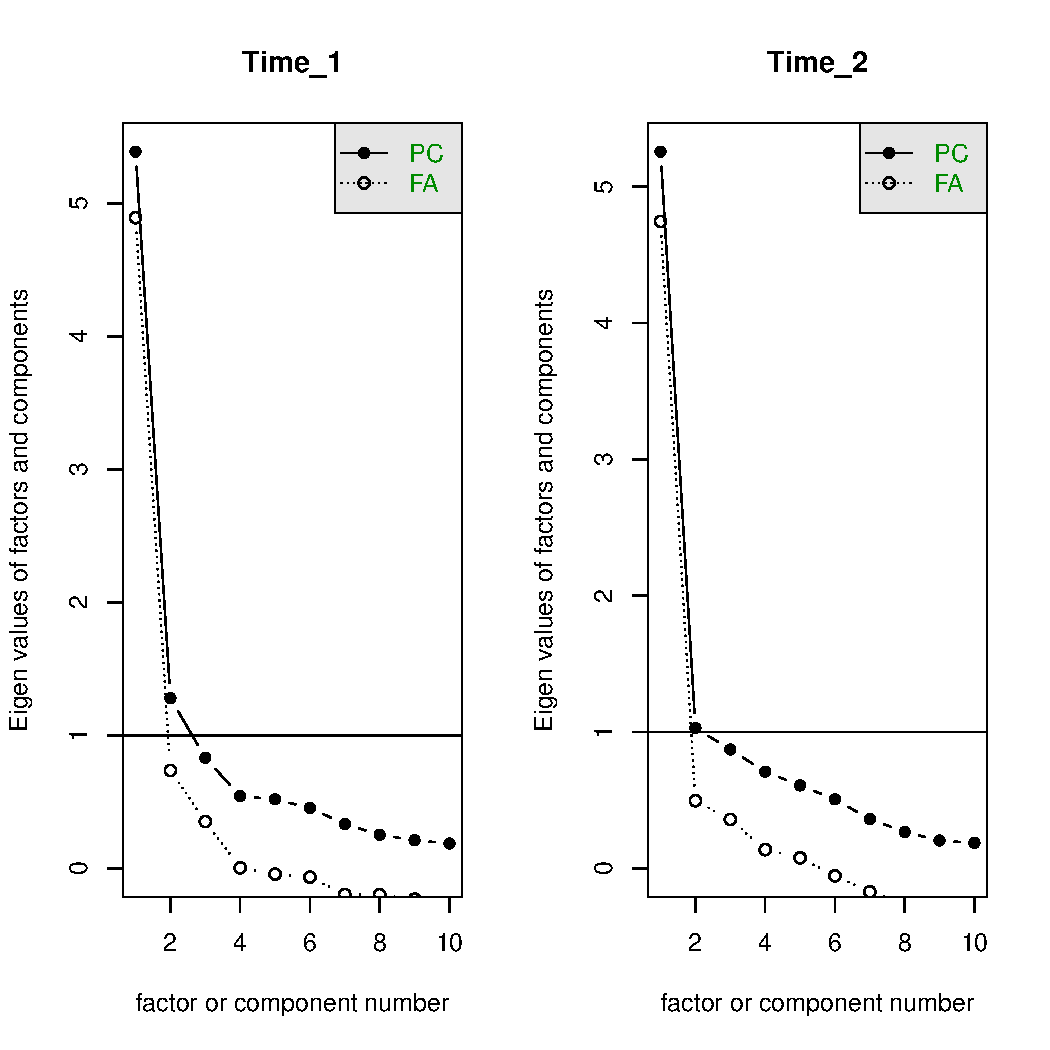
\includegraphics[width=\maxwidth]{figure/unnamed-chunk-4-1} 
\begin{kframe}\begin{verbatim}
## # A tibble: 2 x 3
##   time   data                  scree      
##   <chr>  <list>                <list>     
## 1 Time_1 <tibble [1,000 x 10]> <S3: psych>
## 2 Time_2 <tibble [1,000 x 10]> <S3: psych>
\end{verbatim}
\end{kframe}
\end{knitrout}

The scree test suggests 2 components at time 1 and 2.  

\subsection{Parallel Analysis}
\begin{knitrout}
\definecolor{shadecolor}{rgb}{0.969, 0.969, 0.969}\color{fgcolor}\begin{kframe}
\begin{alltt}
\hlstd{nested_dat} \hlopt
  \hlkwd{mutate}\hlstd{(}\hlkwc{parallel} \hlstd{=} \hlkwd{map2}\hlstd{(data, time,} \hlopt{~}\hlkwd{fa.parallel}\hlstd{(.x,} \hlkwc{main} \hlstd{= .y,} \hlkwc{fa} \hlstd{=} \hlstr{"pc"}\hlstd{)))}
\end{alltt}
\end{kframe}
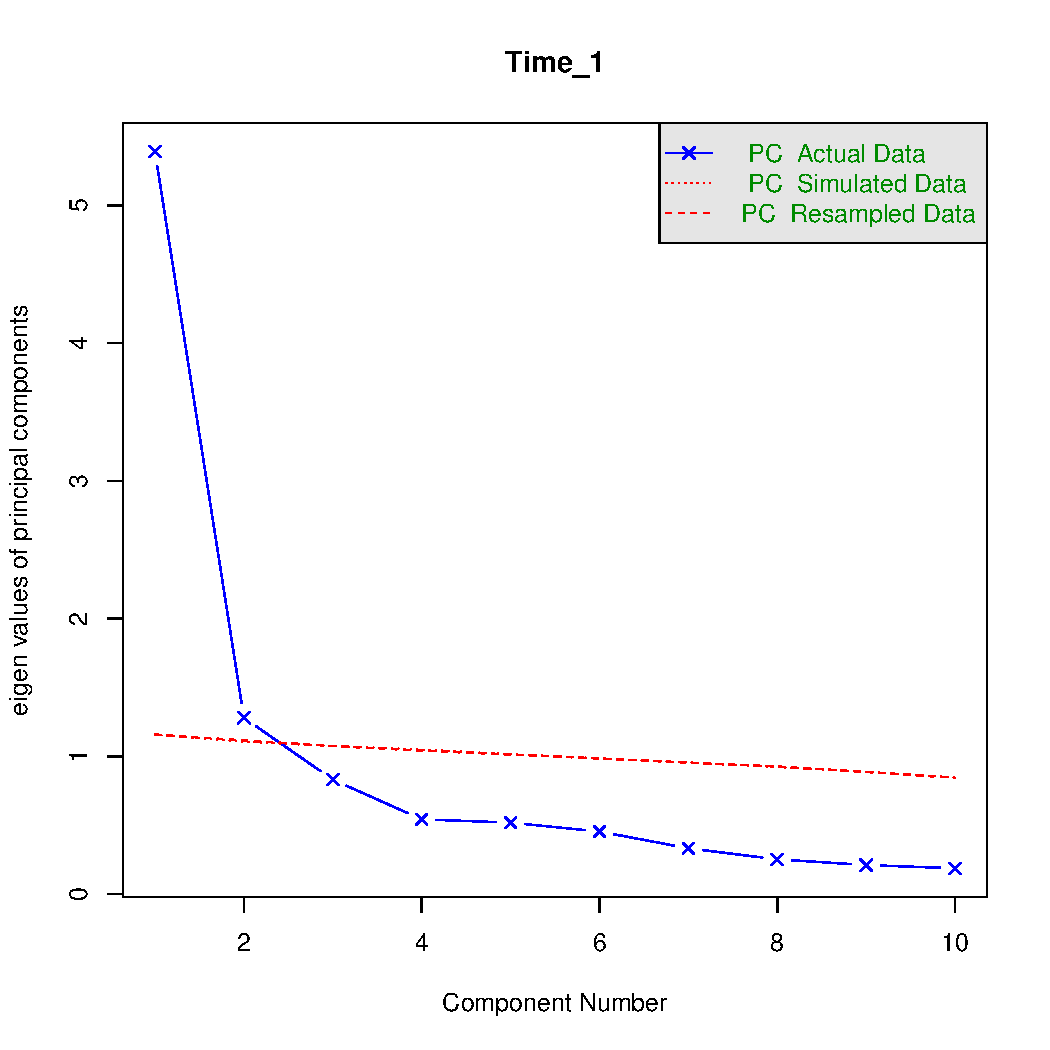
\includegraphics[width=\maxwidth]{figure/unnamed-chunk-5-1} 
\begin{kframe}\begin{verbatim}
## Parallel analysis suggests that the number of factors =  NA  and the number of components =  2
\end{verbatim}
\end{kframe}
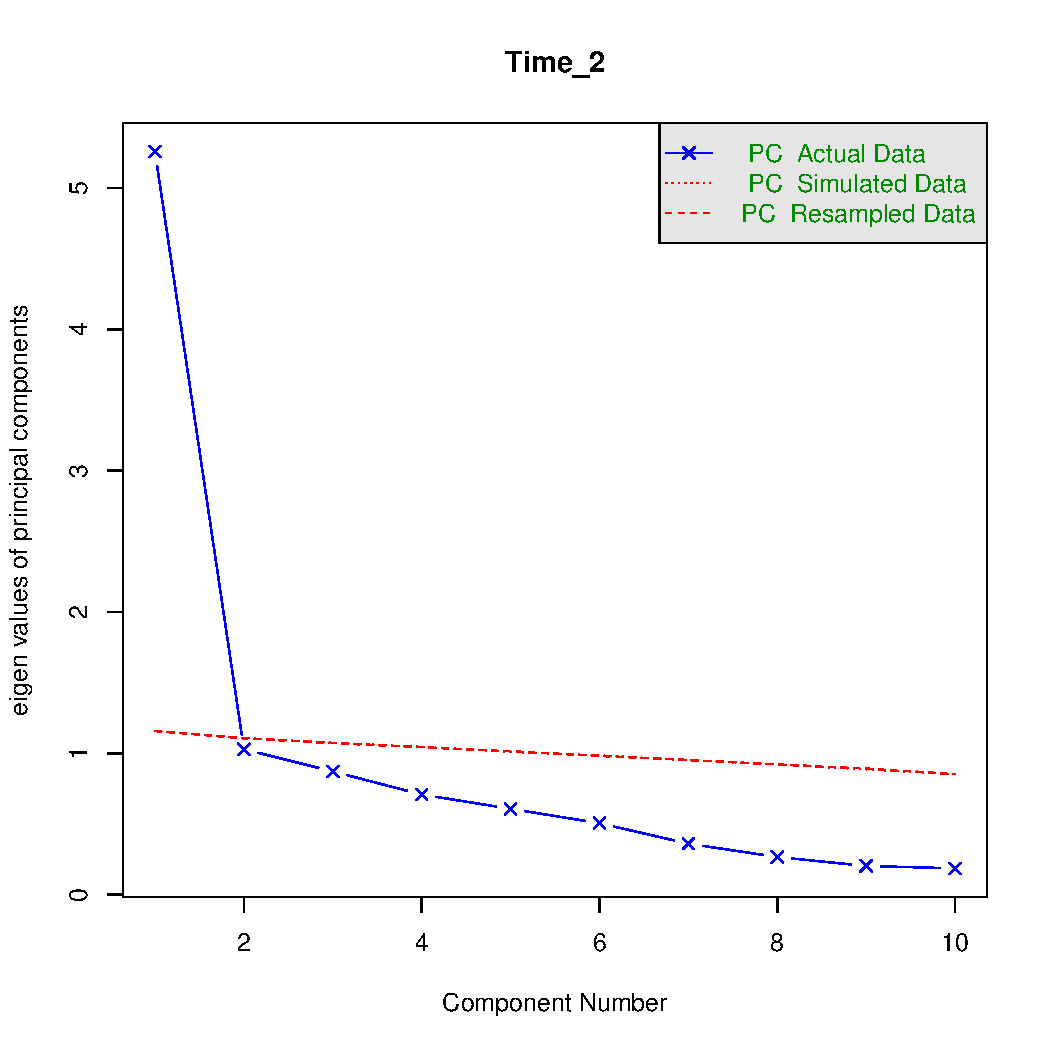
\includegraphics[width=\maxwidth]{figure/unnamed-chunk-5-2} 
\begin{kframe}\begin{verbatim}
## Parallel analysis suggests that the number of factors =  NA  and the number of components =  1
## # A tibble: 2 x 3
##   time   data                  parallel   
##   <chr>  <list>                <list>     
## 1 Time_1 <tibble [1,000 x 10]> <S3: psych>
## 2 Time_2 <tibble [1,000 x 10]> <S3: psych>
\end{verbatim}
\end{kframe}
\end{knitrout}

Paralell analysis suggests 2 components at time 1 and 1 at time 2.

\subsection{Very Simple Structure (VSS)}
\begin{knitrout}
\definecolor{shadecolor}{rgb}{0.969, 0.969, 0.969}\color{fgcolor}\begin{kframe}
\begin{alltt}
\hlkwd{par}\hlstd{(}\hlkwc{mfrow}\hlstd{=}\hlkwd{c}\hlstd{(}\hlnum{1}\hlstd{,}\hlnum{1}\hlstd{))}
\hlstd{nested_dat} \hlkwb{<-} \hlstd{nested_dat} \hlopt
  \hlkwd{mutate}\hlstd{(}\hlkwc{vss} \hlstd{=} \hlkwd{map2}\hlstd{(data, time,} \hlopt{~}\hlkwd{vss}\hlstd{(.x,} \hlkwc{n} \hlstd{=} \hlnum{10}\hlstd{,} \hlkwc{rotate} \hlstd{=} \hlstr{"none"}\hlstd{,} \hlkwc{title} \hlstd{= .y,} \hlkwc{fm} \hlstd{=} \hlstr{"pc"}\hlstd{)))}
\end{alltt}
\end{kframe}
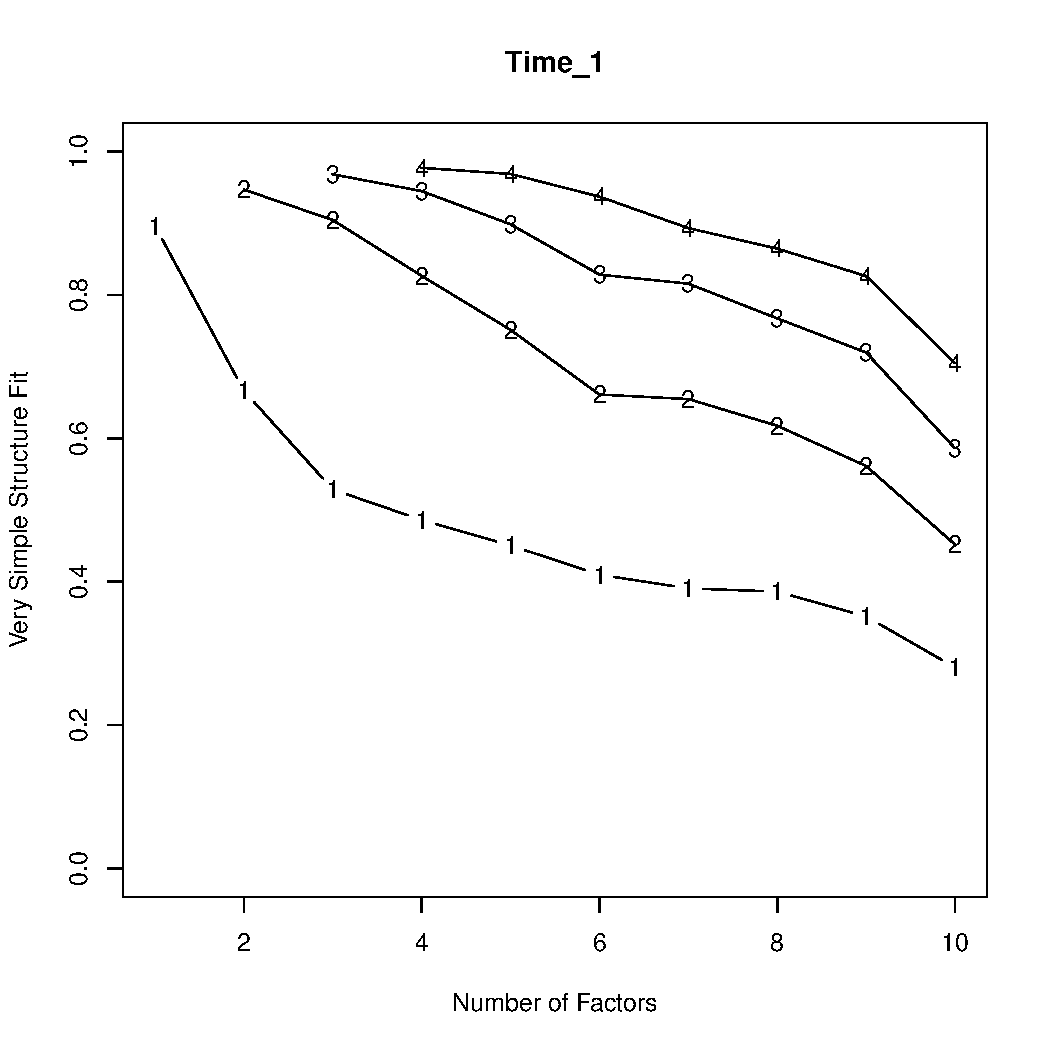
\includegraphics[width=\maxwidth]{figure/unnamed-chunk-6-1} 

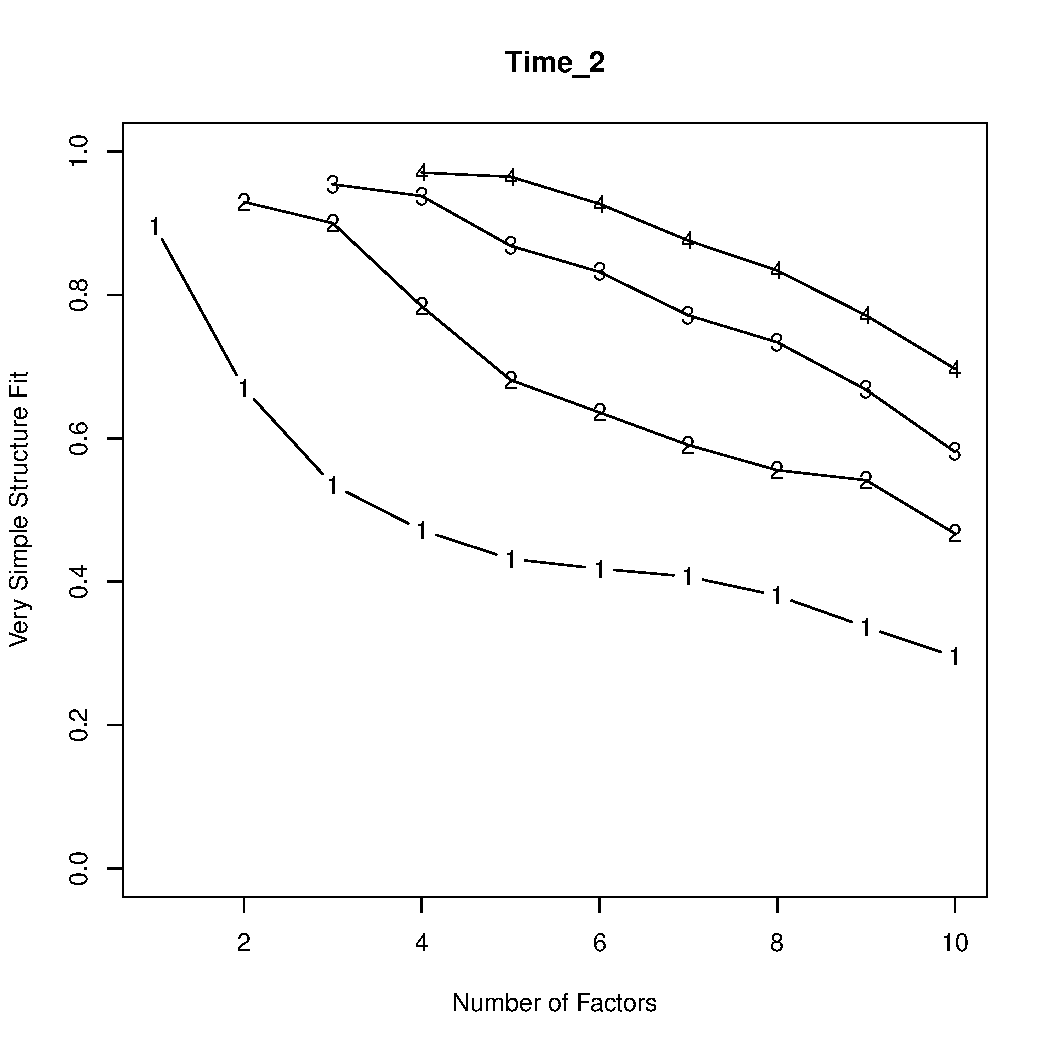
\includegraphics[width=\maxwidth]{figure/unnamed-chunk-6-2} 

\end{knitrout}

VSS seems to suggest 3 factors are optimal at both times.  

\subsection{Minimum Average Partial (MAP)}
\begin{knitrout}
\definecolor{shadecolor}{rgb}{0.969, 0.969, 0.969}\color{fgcolor}\begin{kframe}
\begin{alltt}
\hlstd{map_fun} \hlkwb{<-} \hlkwa{function}\hlstd{(}\hlkwc{v}\hlstd{)\{}
  \hlkwd{data.frame}\hlstd{(v}\hlopt{$}\hlstd{map)} \hlopt \hlkwd{mutate}\hlstd{(}\hlkwc{Component} \hlstd{=} \hlnum{1}\hlopt{:}\hlkwd{nrow}\hlstd{(.))} \hlopt
    \hlkwd{setNames}\hlstd{(}\hlkwd{c}\hlstd{(}\hlstr{"MAP"}\hlstd{,} \hlstr{"Component"}\hlstd{))}
\hlstd{\}}
\hlstd{nested_dat} \hlopt
  \hlkwd{mutate}\hlstd{(}\hlkwc{map} \hlstd{=} \hlkwd{map}\hlstd{(vss, map_fun))} \hlopt
  \hlkwd{unnest}\hlstd{(map)} \hlopt
  \hlkwd{group_by}\hlstd{(time)} \hlopt
  \hlkwd{mutate}\hlstd{(}\hlkwc{min} \hlstd{=} \hlkwd{ifelse}\hlstd{(MAP} \hlopt{==} \hlkwd{min}\hlstd{(MAP,} \hlkwc{na.rm} \hlstd{= T),} \hlstr{"NC"}\hlstd{,} \hlstr{"No"}\hlstd{))} \hlopt
  \hlkwd{ggplot}\hlstd{(}\hlkwd{aes}\hlstd{(}\hlkwc{x} \hlstd{= Component,} \hlkwc{y} \hlstd{= MAP,} \hlkwc{shape} \hlstd{= time))} \hlopt{+}
  \hlkwd{scale_size_manual}\hlstd{(}\hlkwc{values} \hlstd{=} \hlkwd{c}\hlstd{(}\hlnum{3}\hlstd{,} \hlnum{1}\hlstd{))} \hlopt{+}
  \hlkwd{geom_line}\hlstd{()} \hlopt{+}
  \hlkwd{geom_point}\hlstd{(}\hlkwd{aes}\hlstd{(}\hlkwc{size} \hlstd{= min))} \hlopt{+}
  \hlkwd{facet_grid}\hlstd{(}\hlopt{~}\hlstd{time)} \hlopt{+}
  \hlkwd{theme_classic}\hlstd{()} \hlopt{+}
  \hlkwd{theme}\hlstd{(}\hlkwc{legend.position} \hlstd{=} \hlstr{"none"}\hlstd{)}
\end{alltt}
\end{kframe}
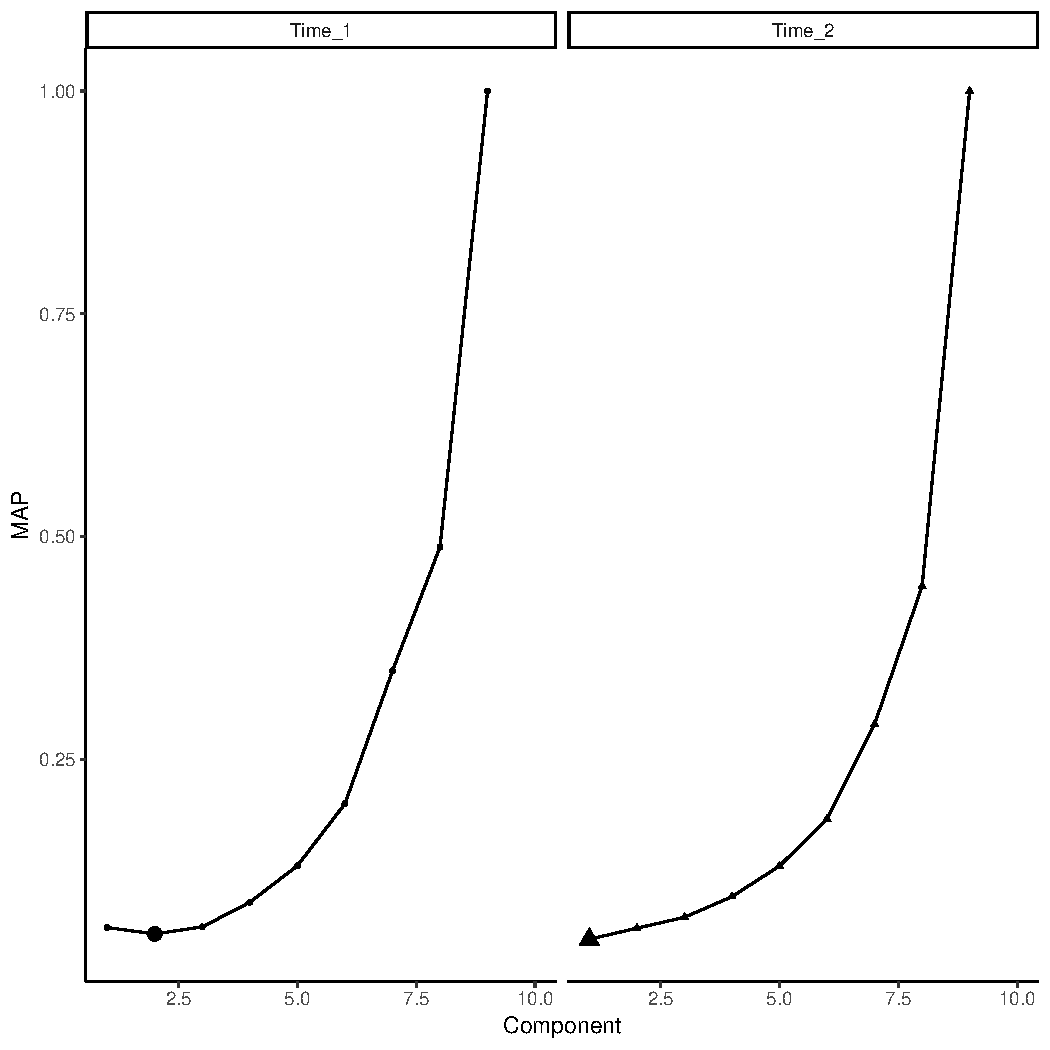
\includegraphics[width=\maxwidth]{figure/unnamed-chunk-7-1} 

\end{knitrout}

The MAP test suggests 2 components at time 1 and 1 at time 2.  

\textcolor{blue}{Overall, the tests seem to suggest 2 components at time 1 and 1 at time 2}.

\section{Question 2}
Now conduct a principal components analysis on each set of 10 items, extract three principal components from each set, and save the unrotated principal component scores. Calculate the correlations among the combined set of principal component scores (this will be a 6 x 6 matrix).
\begin{knitrout}
\definecolor{shadecolor}{rgb}{0.969, 0.969, 0.969}\color{fgcolor}\begin{kframe}
\begin{alltt}
\hlstd{nested_dat} \hlkwb{<-} \hlstd{nested_dat} \hlopt
  \hlkwd{mutate}\hlstd{(}\hlkwc{pc} \hlstd{=} \hlkwd{map}\hlstd{(data,} \hlopt{~}\hlkwd{principal}\hlstd{(.,} \hlkwc{nfactors} \hlstd{=} \hlnum{3}\hlstd{,} \hlkwc{rotate} \hlstd{=} \hlstr{"none"}\hlstd{,} \hlkwc{scores} \hlstd{=} \hlnum{TRUE}\hlstd{)),}
         \hlkwc{scores} \hlstd{=} \hlkwd{map}\hlstd{(pc,} \hlopt{~}\hlkwd{as.tibble}\hlstd{(.}\hlopt{$}\hlstd{scores)))}

\hlstd{tmp2} \hlkwb{<-} \hlstd{nested_dat} \hlopt \hlkwd{unnest}\hlstd{(scores)} \hlopt
  \hlkwd{group_by}\hlstd{(time)} \hlopt
  \hlkwd{mutate}\hlstd{(}\hlkwc{SID} \hlstd{=} \hlnum{1}\hlopt{:}\hlkwd{n}\hlstd{())} \hlopt
  \hlkwd{gather}\hlstd{(}\hlkwc{key} \hlstd{= item,} \hlkwc{value} \hlstd{= value,} \hlopt{-}\hlstd{time,} \hlopt{-}\hlstd{SID)} \hlopt
  \hlkwd{unite}\hlstd{(tmp, time, item,} \hlkwc{sep} \hlstd{=} \hlstr{"."}\hlstd{)} \hlopt
  \hlkwd{spread}\hlstd{(tmp, value)}
\end{alltt}
\end{kframe}
\end{knitrout}



\subsection{Part A}
What are the correlations for corresponding component scores (Time 1 and Time 2)?
\begin{knitrout}
\definecolor{shadecolor}{rgb}{0.969, 0.969, 0.969}\color{fgcolor}\begin{kframe}
\begin{alltt}
\hlkwd{cor}\hlstd{(tmp2} \hlopt \hlkwd{select}\hlstd{(Time_1.PC1}\hlopt{:}\hlstd{Time_1.PC3), tmp2} \hlopt \hlkwd{select}\hlstd{(Time_2.PC1}\hlopt{:}\hlstd{Time_2.PC3))} \hlopt
  \hlkwd{kable}\hlstd{(.,} \hlstr{"latex"}\hlstd{,} \hlkwc{row.names} \hlstd{= F,} \hlkwc{digits} \hlstd{=} \hlnum{2}\hlstd{,}
        \hlkwc{col.names} \hlstd{=} \hlkwd{c}\hlstd{(}\hlstr{"PC1"}\hlstd{,} \hlstr{"PC2"}\hlstd{,} \hlstr{"PC3"}\hlstd{))} \hlopt
  \hlkwd{add_header_above}\hlstd{(}\hlkwd{c}\hlstd{(}\hlstr{"Time 2"} \hlstd{=} \hlnum{3}\hlstd{))} \hlopt
  \hlkwd{group_rows}\hlstd{(}\hlstr{"Time 1"}\hlstd{,} \hlnum{1}\hlstd{,} \hlnum{3}\hlstd{)}
\end{alltt}
\end{kframe}
\begin{tabular}{r|r|r}
\hline
\multicolumn{3}{|c}{Time 2} \\
\cline{1-3}
PC1 & PC2 & PC3\\
\hline
\multicolumn{3}{l}{\textbf{Time 1}}\\
\hline
\hspace{1em}0.84 & 0.00 & 0.04\\
\hline
\hspace{1em}0.15 & -0.38 & -0.09\\
\hline
\hspace{1em}0.04 & 0.10 & -0.22\\
\hline
\end{tabular}


\end{knitrout}

 
\subsection{Part B}
The magnitudes of these correlations will be related to the magnitudes of the component eigenvalues. Why does this make sense?  

Eigenvalues represent the variances of the components, so the scores should capture much of the variance of the components. 
 
\section{Question 3}
Repeat the analyses, but now rotate to simple structure in the two sets using varimax rotation. Save the rotated principal component scores and examine the intercorrelations.
\begin{knitrout}
\definecolor{shadecolor}{rgb}{0.969, 0.969, 0.969}\color{fgcolor}\begin{kframe}
\begin{alltt}
\hlstd{nested_dat} \hlkwb{<-} \hlstd{nested_dat} \hlopt
  \hlkwd{mutate}\hlstd{(}\hlkwc{pc.vm} \hlstd{=} \hlkwd{map}\hlstd{(data,} \hlopt{~}\hlkwd{principal}\hlstd{(.,} \hlkwc{nfactors} \hlstd{=} \hlnum{3}\hlstd{,} \hlkwc{rotate} \hlstd{=} \hlstr{"varimax"}\hlstd{,} \hlkwc{scores} \hlstd{=} \hlnum{TRUE}\hlstd{)),}
         \hlkwc{scores.vm} \hlstd{=} \hlkwd{map}\hlstd{(pc.vm,} \hlopt{~}\hlkwd{as.tibble}\hlstd{(.}\hlopt{$}\hlstd{scores)))}

\hlstd{tmp3} \hlkwb{<-} \hlstd{nested_dat} \hlopt \hlkwd{unnest}\hlstd{(scores.vm)} \hlopt
  \hlkwd{group_by}\hlstd{(time)} \hlopt
  \hlkwd{mutate}\hlstd{(}\hlkwc{SID} \hlstd{=} \hlnum{1}\hlopt{:}\hlkwd{n}\hlstd{())} \hlopt
  \hlkwd{gather}\hlstd{(}\hlkwc{key} \hlstd{= item,} \hlkwc{value} \hlstd{= value,} \hlopt{-}\hlstd{time,} \hlopt{-}\hlstd{SID)} \hlopt
  \hlkwd{unite}\hlstd{(tmp, time, item,} \hlkwc{sep} \hlstd{=} \hlstr{"."}\hlstd{)} \hlopt
  \hlkwd{spread}\hlstd{(tmp, value)}
\end{alltt}
\end{kframe}
\end{knitrout}


\subsection{Part A}
Do the principal components from Time 1 replicate at Time 2? 
\begin{knitrout}
\definecolor{shadecolor}{rgb}{0.969, 0.969, 0.969}\color{fgcolor}\begin{kframe}
\begin{alltt}
\hlkwd{cor}\hlstd{(tmp3} \hlopt \hlkwd{select}\hlstd{(Time_1.RC1}\hlopt{:}\hlstd{Time_1.RC3), tmp3} \hlopt \hlkwd{select}\hlstd{(Time_2.RC1}\hlopt{:}\hlstd{Time_2.RC3))} \hlopt
  \hlkwd{kable}\hlstd{(.,} \hlstr{"latex"}\hlstd{,} \hlkwc{row.names} \hlstd{= F,} \hlkwc{digits} \hlstd{=} \hlnum{2}\hlstd{,}
        \hlkwc{col.names} \hlstd{=} \hlkwd{c}\hlstd{(}\hlstr{"PC1"}\hlstd{,} \hlstr{"PC2"}\hlstd{,} \hlstr{"PC3"}\hlstd{))} \hlopt
  \hlkwd{add_header_above}\hlstd{(}\hlkwd{c}\hlstd{(}\hlstr{"Time 2"} \hlstd{=} \hlnum{3}\hlstd{))} \hlopt
  \hlkwd{group_rows}\hlstd{(}\hlstr{"Time 1"}\hlstd{,} \hlnum{1}\hlstd{,} \hlnum{3}\hlstd{)}
\end{alltt}
\end{kframe}
\begin{tabular}{r|r|r}
\hline
\multicolumn{3}{|c}{Time 2} \\
\cline{1-3}
PC1 & PC2 & PC3\\
\hline
\multicolumn{3}{l}{\textbf{Time 1}}\\
\hline
\hspace{1em}0.11 & 0.30 & 0.35\\
\hline
\hspace{1em}0.58 & 0.02 & 0.32\\
\hline
\hspace{1em}0.32 & 0.41 & 0.10\\
\hline
\end{tabular}


\end{knitrout}

No, the highest correlation between any 2 given factors is .66. Indeed, the third component at the second time point does not strongly resemble any component at time 1.
\subsection{Part B}
Why?

The correlation between factor scores at the different times is weak. The second component at time 1 appears to resemble the first component at time 2 (r = .66), but it's not clear that the 1st or 3rd components in wave are reflected in any of the components at wave 2. \textcolor{blue}{This likely occurs because the 1st and 3rd factors are not "real." It's also possible although unlikely that something happened over the four week period that changed the structure of self-esteem among the students.}

\section{Question 4}
Repeat the analysis from Question 3, but now use factor analysis (set the factor method option to maximum likelihood, fm="ml"; you might also need to increase the number of iterations).
\begin{knitrout}
\definecolor{shadecolor}{rgb}{0.969, 0.969, 0.969}\color{fgcolor}\begin{kframe}
\begin{alltt}
\hlstd{nested_dat} \hlkwb{<-} \hlstd{nested_dat} \hlopt
  \hlkwd{mutate}\hlstd{(}\hlkwc{fa} \hlstd{=} \hlkwd{map}\hlstd{(data,} \hlopt{~}\hlkwd{fa}\hlstd{(.,} \hlkwc{nfactors} \hlstd{=} \hlnum{3}\hlstd{,} \hlkwc{rotate} \hlstd{=} \hlstr{"varimax"}\hlstd{,} \hlkwc{scores} \hlstd{=} \hlnum{TRUE}\hlstd{,} \hlkwc{fm} \hlstd{=} \hlstr{"ml"}\hlstd{)),}
         \hlkwc{scores.fa} \hlstd{=} \hlkwd{map}\hlstd{(pc.vm,} \hlopt{~}\hlkwd{as.tibble}\hlstd{(.}\hlopt{$}\hlstd{scores)))}
\end{alltt}
\end{kframe}
\end{knitrout}


\subsection{Part A}
(a) How does this affect the eigenvalues for the extracted linear combinations? 
\begin{knitrout}
\definecolor{shadecolor}{rgb}{0.969, 0.969, 0.969}\color{fgcolor}\begin{kframe}
\begin{alltt}
\hlkwd{tibble}\hlstd{(}
  \hlkwc{fa_1} \hlstd{= nested_dat}\hlopt{$}\hlstd{fa[[}\hlnum{1}\hlstd{]]}\hlopt{$}\hlstd{values,}
  \hlkwc{pca_1} \hlstd{= nested_dat}\hlopt{$}\hlstd{pc.vm[[}\hlnum{1}\hlstd{]]}\hlopt{$}\hlstd{values,}
  \hlkwc{fa_2} \hlstd{= nested_dat}\hlopt{$}\hlstd{fa[[}\hlnum{2}\hlstd{]]}\hlopt{$}\hlstd{values,}
  \hlkwc{pca_2} \hlstd{= nested_dat}\hlopt{$}\hlstd{pc.vm[[}\hlnum{2}\hlstd{]]}\hlopt{$}\hlstd{values)}
\end{alltt}
\begin{verbatim}
## # A tibble: 10 x 4
##          fa_1 pca_1    fa_2 pca_2
##         <dbl> <dbl>   <dbl> <dbl>
##  1  5.06      5.39   4.91   5.26 
##  2  0.988     1.28   0.743  1.03 
##  3  0.521     0.831  0.600  0.872
##  4  0.100     0.543  0.194  0.709
##  5  0.0762    0.519  0.145  0.608
##  6  0.0249    0.454  0.0542 0.506
##  7 -0.0000531 0.333 -0.0114 0.361
##  8 -0.00198   0.252 -0.0675 0.267
##  9 -0.0371    0.211 -0.0996 0.203
## 10 -0.172     0.187 -0.215  0.187
\end{verbatim}
\begin{alltt}
\hlstd{nested_dat}\hlopt{$}\hlstd{fa[[}\hlnum{2}\hlstd{]]}\hlopt{$}\hlstd{values}
\end{alltt}
\begin{verbatim}
##  [1]  4.91296929  0.74344285  0.60031952  0.19421193  0.14461595
##  [6]  0.05419439 -0.01144530 -0.06754470 -0.09958244 -0.21451904
\end{verbatim}
\end{kframe}
\end{knitrout}

Some of the eigenvalues are now negative \textcolor{blue}{and are overall smaller in magnitude}. 

\subsection{Part B}
What happens to the pattern of correlations among factor scores?
\begin{knitrout}
\definecolor{shadecolor}{rgb}{0.969, 0.969, 0.969}\color{fgcolor}\begin{kframe}
\begin{alltt}
\hlstd{tmp4} \hlkwb{<-} \hlstd{nested_dat} \hlopt \hlkwd{unnest}\hlstd{(scores.fa)} \hlopt
  \hlkwd{group_by}\hlstd{(time)} \hlopt
  \hlkwd{mutate}\hlstd{(}\hlkwc{SID} \hlstd{=} \hlnum{1}\hlopt{:}\hlkwd{n}\hlstd{())} \hlopt
  \hlkwd{gather}\hlstd{(}\hlkwc{key} \hlstd{= item,} \hlkwc{value} \hlstd{= value,} \hlopt{-}\hlstd{time,} \hlopt{-}\hlstd{SID)} \hlopt
  \hlkwd{unite}\hlstd{(tmp, time, item,} \hlkwc{sep} \hlstd{=} \hlstr{"."}\hlstd{)} \hlopt
  \hlkwd{spread}\hlstd{(tmp, value)}

\hlkwd{cor}\hlstd{(tmp4} \hlopt \hlkwd{select}\hlstd{(Time_1.RC1}\hlopt{:}\hlstd{Time_1.RC3), tmp4} \hlopt \hlkwd{select}\hlstd{(Time_2.RC1}\hlopt{:}\hlstd{Time_2.RC3))} \hlopt
  \hlkwd{kable}\hlstd{(.,} \hlstr{"latex"}\hlstd{,} \hlkwc{row.names} \hlstd{= F,} \hlkwc{digits} \hlstd{=} \hlnum{2}\hlstd{,}
        \hlkwc{col.names} \hlstd{=} \hlkwd{c}\hlstd{(}\hlstr{"PC1"}\hlstd{,} \hlstr{"PC2"}\hlstd{,} \hlstr{"PC3"}\hlstd{))} \hlopt
  \hlkwd{add_header_above}\hlstd{(}\hlkwd{c}\hlstd{(}\hlstr{"Time 2"} \hlstd{=} \hlnum{3}\hlstd{))} \hlopt
  \hlkwd{group_rows}\hlstd{(}\hlstr{"Time 1"}\hlstd{,} \hlnum{1}\hlstd{,} \hlnum{3}\hlstd{)}
\end{alltt}
\end{kframe}
\begin{tabular}{r|r|r}
\hline
\multicolumn{3}{|c}{Time 2} \\
\cline{1-3}
PC1 & PC2 & PC3\\
\hline
\multicolumn{3}{l}{\textbf{Time 1}}\\
\hline
\hspace{1em}0.11 & 0.30 & 0.35\\
\hline
\hspace{1em}0.58 & 0.02 & 0.32\\
\hline
\hspace{1em}0.32 & 0.41 & 0.10\\
\hline
\end{tabular}


\end{knitrout}

They appear unaffected. At best, only one factor appears to replicate. 

\section{Question 5}
What does this series of analyses tell you about the stability of principal components and factor scores, the hazards of overfactoring, and the importance of replication before trusting the meaning and interpretation of scores?

This analysis suggests that principle components and factor scores may, in some circumstances, be dubiously related over time. Moreover, the more factors that are extracted, the less likely they are to replicate. This likely occurs becuase although additional factors explain more of the total variance, the propotion of variance they explain are much smaller than previously extracted factors. In this case, at best one factor appears to be stable at all, despite the fact that the various methods for testing the needed number of factors suggested 2 factors were needed. 

\end{document}
